%% bare_conf.tex
%% V1.3
%% 2007/01/11
%% by Michael Shell
%% See:
%% http://www.michaelshell.org/
%% for current contact information.
%%
%% This is a skeleton file demonstrating the use of IEEEtran.cls
%% (requires IEEEtran.cls version 1.7 or later) with an IEEE conference paper.
%%
%% Support sites:
%% http://www.michaelshell.org/tex/ieeetran/
%% http://www.ctan.org/tex-archive/macros/latex/contrib/IEEEtran/
%% and
%% http://www.ieee.org/

%%*************************************************************************
%% Legal Notice:
%% This code is offered as-is without any warranty either expressed or
%% implied; without even the implied warranty of MERCHANTABILITY or
%% FITNESS FOR A PARTICULAR PURPOSE! 
%% User assumes all risk.
%% In no event shall IEEE or any contributor to this code be liable for
%% any damages or losses, including, but not limited to, incidental,
%% consequential, or any other damages, resulting from the use or misuse
%% of any information contained here.
%%
%% All comments are the opinions of their respective authors and are not
%% necessarily endorsed by the IEEE.
%%
%% This work is distributed under the LaTeX Project Public License (LPPL)
%% ( http://www.latex-project.org/ ) version 1.3, and may be freely used,
%% distributed and modified. A copy of the LPPL, version 1.3, is included
%% in the base LaTeX documentation of all distributions of LaTeX released
%% 2003/12/01 or later.
%% Retain all contribution notices and credits.
%% ** Modified files should be clearly indicated as such, including  **
%% ** renaming them and changing author support contact information. **
%%
%% File list of work: IEEEtran.cls, IEEEtran_HOWTO.pdf, bare_adv.tex,
%%                    bare_conf.tex, bare_jrnl.tex, bare_jrnl_compsoc.tex
%%*************************************************************************

% *** Authors should verify (and, if needed, correct) their LaTeX system  ***
% *** with the testflow diagnostic prior to trusting their LaTeX platform ***
% *** with production work. IEEE's font choices can trigger bugs that do  ***
% *** not appear when using other class files.                            ***
% The testflow support page is at:
% http://www.michaelshell.org/tex/testflow/



% Note that the a4paper option is mainly intended so that authors in
% countries using A4 can easily print to A4 and see how their papers will
% look in print - the typesetting of the document will not typically be
% affected with changes in paper size (but the bottom and side margins will).
% Use the testflow package mentioned above to verify correct handling of
% both paper sizes by the user's LaTeX system.
%
% Also note that the "draftcls" or "draftclsnofoot", not "draft", option
% should be used if it is desired that the figures are to be displayed in
% draft mode.
%
\documentclass[10pt,final,journal,a4paper]{IEEEtran}
% Add the compsoc option for Computer Society conferences.
%
% If IEEEtran.cls has not been installed into the LaTeX system files,
% manually specify the path to it like:
% \documentclass[conference]{../sty/IEEEtran}





% Some very useful LaTeX packages include:
% (uncomment the ones you want to load)


% *** MISC UTILITY PACKAGES ***
%
%\usepackage{ifpdf}
% Heiko Oberdiek's ifpdf.sty is very useful if you need conditional
% compilation based on whether the output is pdf or dvi.
% usage:
% \ifpdf
%   % pdf code
% \else
%   % dvi code
% \fi
% The latest version of ifpdf.sty can be obtained from:
% http://www.ctan.org/tex-archive/macros/latex/contrib/oberdiek/
% Also, note that IEEEtran.cls V1.7 and later provides a builtin
% \ifCLASSINFOpdf conditional that works the same way.
% When switching from latex to pdflatex and vice-versa, the compiler may
% have to be run twice to clear warning/error messages.






% *** CITATION PACKAGES ***
%
\usepackage{cite}
% cite.sty was written by Donald Arseneau
% V1.6 and later of IEEEtran pre-defines the format of the cite.sty package
% \cite{} output to follow that of IEEE. Loading the cite package will
% result in citation numbers being automatically sorted and properly
% "compressed/ranged". e.g., [1], [9], [2], [7], [5], [6] without using
% cite.sty will become [1], [2], [5]--[7], [9] using cite.sty. cite.sty's
% \cite will automatically add leading space, if needed. Use cite.sty's
% noadjust option (cite.sty V3.8 and later) if you want to turn this off.
% cite.sty is already installed on most LaTeX systems. Be sure and use
% version 4.0 (2003-05-27) and later if using hyperref.sty. cite.sty does
% not currently provide for hyperlinked citations.
% The latest version can be obtained at:
% http://www.ctan.org/tex-archive/macros/latex/contrib/cite/
% The documentation is contained in the cite.sty file itself.






% *** GRAPHICS RELATED PACKAGES ***
%
\ifCLASSINFOpdf
  % \usepackage[pdftex]{graphicx}
  % declare the path(s) where your graphic files are
  % \graphicspath{{../pdf/}{../jpeg/}}
  % and their extensions so you won't have to specify these with
  % every instance of \includegraphics
  % \DeclareGraphicsExtensions{.pdf,.jpeg,.png}
\else
  % or other class option (dvipsone, dvipdf, if not using dvips). graphicx
  % will default to the driver specified in the system graphics.cfg if no
  % driver is specified.
  % \usepackage[dvips]{graphicx}
  % declare the path(s) where your graphic files are
  % \graphicspath{{../eps/}}
  % and their extensions so you won't have to specify these with
  % every instance of \includegraphics
  % \DeclareGraphicsExtensions{.eps}
\fi
% graphicx was written by David Carlisle and Sebastian Rahtz. It is
% required if you want graphics, photos, etc. graphicx.sty is already
% installed on most LaTeX systems. The latest version and documentation can
% be obtained at: 
% http://www.ctan.org/tex-archive/macros/latex/required/graphics/
% Another good source of documentation is "Using Imported Graphics in
% LaTeX2e" by Keith Reckdahl which can be found as epslatex.ps or
% epslatex.pdf at: http://www.ctan.org/tex-archive/info/
%
% latex, and pdflatex in dvi mode, support graphics in encapsulated
% postscript (.eps) format. pdflatex in pdf mode supports graphics
% in .pdf, .jpeg, .png and .mps (metapost) formats. Users should ensure
% that all non-photo figures use a vector format (.eps, .pdf, .mps) and
% not a bitmapped formats (.jpeg, .png). IEEE frowns on bitmapped formats
% which can result in "jaggedy"/blurry rendering of lines and letters as
% well as large increases in file sizes.
%
% You can find documentation about the pdfTeX application at:
% http://www.tug.org/applications/pdftex





% *** MATH PACKAGES ***
%
\usepackage[cmex10]{amsmath}
% A popular package from the American Mathematical Society that provides
% many useful and powerful commands for dealing with mathematics. If using
% it, be sure to load this package with the cmex10 option to ensure that
% only type 1 fonts will utilized at all point sizes. Without this option,
% it is possible that some math symbols, particularly those within
% footnotes, will be rendered in bitmap form which will result in a
% document that can not be IEEE Xplore compliant!
%
% Also, note that the amsmath package sets \interdisplaylinepenalty to 10000
% thus preventing page breaks from occurring within multiline equations. Use:
%\interdisplaylinepenalty=2500
% after loading amsmath to restore such page breaks as IEEEtran.cls normally
% does. amsmath.sty is already installed on most LaTeX systems. The latest
% version and documentation can be obtained at:
% http://www.ctan.org/tex-archive/macros/latex/required/amslatex/math/





% *** SPECIALIZED LIST PACKAGES ***
%
\usepackage{algorithmic}
% algorithmic.sty was written by Peter Williams and Rogerio Brito.
% This package provides an algorithmic environment fo describing algorithms.
% You can use the algorithmic environment in-text or within a figure
% environment to provide for a floating algorithm. Do NOT use the algorithm
% floating environment provided by algorithm.sty (by the same authors) or
% algorithm2e.sty (by Christophe Fiorio) as IEEE does not use dedicated
% algorithm float types and packages that provide these will not provide
% correct IEEE style captions. The latest version and documentation of
% algorithmic.sty can be obtained at:
% http://www.ctan.org/tex-archive/macros/latex/contrib/algorithms/
% There is also a support site at:
% http://algorithms.berlios.de/index.html
% Also of interest may be the (relatively newer and more customizable)
% algorithmicx.sty package by Szasz Janos:
% http://www.ctan.org/tex-archive/macros/latex/contrib/algorithmicx/




% *** ALIGNMENT PACKAGES ***
%
\usepackage{array}
% Frank Mittelbach's and David Carlisle's array.sty patches and improves
% the standard LaTeX2e array and tabular environments to provide better
% appearance and additional user controls. As the default LaTeX2e table
% generation code is lacking to the point of almost being broken with
% respect to the quality of the end results, all users are strongly
% advised to use an enhanced (at the very least that provided by array.sty)
% set of table tools. array.sty is already installed on most systems. The
% latest version and documentation can be obtained at:
% http://www.ctan.org/tex-archive/macros/latex/required/tools/


\usepackage{mdwmath}
\usepackage{mdwtab}
% Also highly recommended is Mark Wooding's extremely powerful MDW tools,
% especially mdwmath.sty and mdwtab.sty which are used to format equations
% and tables, respectively. The MDWtools set is already installed on most
% LaTeX systems. The lastest version and documentation is available at:
% http://www.ctan.org/tex-archive/macros/latex/contrib/mdwtools/


% IEEEtran contains the IEEEeqnarray family of commands that can be used to
% generate multiline equations as well as matrices, tables, etc., of high
% quality.


\usepackage{eqparbox}
% Also of notable interest is Scott Pakin's eqparbox package for creating
% (automatically sized) equal width boxes - aka "natural width parboxes".
% Available at:
% http://www.ctan.org/tex-archive/macros/latex/contrib/eqparbox/





% *** SUBFIGURE PACKAGES ***
%\usepackage[tight,footnotesize]{subfigure}
% subfigure.sty was written by Steven Douglas Cochran. This package makes it
% easy to put subfigures in your figures. e.g., "Figure 1a and 1b". For IEEE
% work, it is a good idea to load it with the tight package option to reduce
% the amount of white space around the subfigures. subfigure.sty is already
% installed on most LaTeX systems. The latest version and documentation can
% be obtained at:
% http://www.ctan.org/tex-archive/obsolete/macros/latex/contrib/subfigure/
% subfigure.sty has been superceeded by subfig.sty.



%\usepackage[caption=false]{caption}
%\usepackage{caption}
%\usepackage[font=footnotesize, captions=false]{subfig}
% subfig.sty, also written by Steven Douglas Cochran, is the modern
% replacement for subfigure.sty. However, subfig.sty requires and
% automatically loads Axel Sommerfeldt's caption.sty which will override
% IEEEtran.cls handling of captions and this will result in nonIEEE style
% figure/table captions. To prevent this problem, be sure and preload
% caption.sty with its "caption=false" package option. This is will preserve
% IEEEtran.cls handing of captions. Version 1.3 (2005/06/28) and later 
% (recommended due to many improvements over 1.2) of subfig.sty supports
% the caption=false option directly:
%\usepackage[caption=false,font=footnotesize]{subfig}
%
% The latest version and documentation can be obtained at:
% http://www.ctan.org/tex-archive/macros/latex/contrib/subfig/
% The latest version and documentation of caption.sty can be obtained at:
% http://www.ctan.org/tex-archive/macros/latex/contrib/caption/




% *** FLOAT PACKAGES ***
%
\usepackage{fixltx2e}
% fixltx2e, the successor to the earlier fix2col.sty, was written by
% Frank Mittelbach and David Carlisle. This package corrects a few problems
% in the LaTeX2e kernel, the most notable of which is that in current
% LaTeX2e releases, the ordering of single and double column floats is not
% guaranteed to be preserved. Thus, an unpatched LaTeX2e can allow a
% single column figure to be placed prior to an earlier double column
% figure. The latest version and documentation can be found at:
% http://www.ctan.org/tex-archive/macros/latex/base/



%\usepackage{stfloats}
% stfloats.sty was written by Sigitas Tolusis. This package gives LaTeX2e
% the ability to do double column floats at the bottom of the page as well
% as the top. (e.g., "\begin{figure*}[!b]" is not normally possible in
% LaTeX2e). It also provides a command:
%\fnbelowfloat
% to enable the placement of footnotes below bottom floats (the standard
% LaTeX2e kernel puts them above bottom floats). This is an invasive package
% which rewrites many portions of the LaTeX2e float routines. It may not work
% with other packages that modify the LaTeX2e float routines. The latest
% version and documentation can be obtained at:
% http://www.ctan.org/tex-archive/macros/latex/contrib/sttools/
% Documentation is contained in the stfloats.sty comments as well as in the
% presfull.pdf file. Do not use the stfloats baselinefloat ability as IEEE
% does not allow \baselineskip to stretch. Authors submitting work to the
% IEEE should note that IEEE rarely uses double column equations and
% that authors should try to avoid such use. Do not be tempted to use the
% cuted.sty or midfloat.sty packages (also by Sigitas Tolusis) as IEEE does
% not format its papers in such ways.





% *** PDF, URL AND HYPERLINK PACKAGES ***
%
\usepackage{url}
% url.sty was written by Donald Arseneau. It provides better support for
% handling and breaking URLs. url.sty is already installed on most LaTeX
% systems. The latest version can be obtained at:
% http://www.ctan.org/tex-archive/macros/latex/contrib/misc/
% Read the url.sty source comments for usage information. Basically,
% \url{my_url_here}.

\usepackage{epsfig}
\usepackage{graphicx}
%\usepackage{subfloat}
%\usepackage{subcaption}
\usepackage[T1]{fontenc}
\usepackage{mwe}
\usepackage{subfig}
\usepackage{float}
%\usepackage{subfloat}
%\usepackage[section]{placeins}

% *** Do not adjust lengths that control margins, column widths, etc. ***
% *** Do not use packages that alter fonts (such as pslatex).         ***
% There should be no need to do such things with IEEEtran.cls V1.6 and later.
% (Unless specifically asked to do so by the journal or conference you plan
% to submit to, of course. )


% correct bad hyphenation here
\hyphenation{op-tical net-works semi-conduc-tor}


\begin{document}
%
% paper title
% can use linebreaks \\ within to get better formatting as desired
\title{Peer-Assisted Content Distribution Aided by Video Popularity Evolution Model}

\author{\IEEEauthorblockN{Mohamad Dikshie Fauzie\IEEEauthorrefmark{1} \quad
Achmad Husni Thamrin\IEEEauthorrefmark{1} \quad
Jun Murai\IEEEauthorrefmark{2}}
\IEEEauthorblockA{\IEEEauthorrefmark{1}Graduate School of Media and Governance} \quad
\IEEEauthorblockA{\IEEEauthorrefmark{2}Faculty of Environment and Information Studies\\ 
Keio University, 252-0882 Kanagawa, Japan \\
dikshie@sfc.wide.ad.jp \quad\quad husni@ai3.net \quad\quad jun@wide.ad.jp}
}




% use for special paper notices
%\IEEEspecialpapernotice{(Invited Paper)}




% make the title area
\maketitle


\begin{abstract}
%\boldmath
Generally content distribution network (CDN) have adopted two different architectures: client-server model that's is the most common architecture model and peer-assisted CDN.  
In client-server model, clients download content dedicated and geographically managed servers while in peer-assisted model, clients download content from each other client.
\end{abstract}
% IEEEtran.cls defaults to using nonbold math in the Abstract.
% This preserves the distinction between vectors and scalars. However,
% if the conference you are submitting to favors bold math in the abstract,
% then you can use LaTeX's standard command \boldmath at the very start
% of the abstract to achieve this. Many IEEE journals/conferences frown on
% math in the abstract anyway.

% no keywords
\begin{IEEEkeywords}
P2P, CDN
\end{IEEEkeywords}





% For peer review papers, you can put extra information on the cover
% page as needed:
% \ifCLASSOPTIONpeerreview
% \begin{center} \bfseries EDICS Category: 3-BBND \end{center}
% \fi
%
% For peerreview papers, this IEEEtran command inserts a page break and
% creates the second title. It will be ignored for other modes.
%\IEEEpeerreviewmaketitle



\section{Introduction}
Streaming content, especially video, represents a significant fraction of the traffic volume on the Internet, and it has become a standard practice to deliver this type of content using Content Delivery Networks (CDNs) such as Akamai and Limelight for better scaling and quality of experience for the end users. 
For example, YouTube uses Google cache and MTV uses Akamai in their operations.

With the spread of broadband Internet access at a reasonable flat monthly rate, users are connected to the Internet 24 hours a day and they can download and share multimedia content. P2P (peer to peer) applications are also widely deployed. 
In China, P2P is very popular; we see many P2P applications from China such as PPLive, PPStream, UUSe, Xunlei, etc. \cite{Vu:2010:UOC:1865106.1865115}. 
Some news broadcasters also rely on P2P technology to deliver popular live events. 
For example, CNN uses the Octoshape \cite{octoshape} solution that enables their broadcast to scale and offer good video quality as the number of users increases.

From the Internet provider point of view, the presence of so many always-on users suggests that it is possible to delegate a portion of computing, storage and networking tasks to the users, thus creating P2P networks where users can share files and multimedia content. 
Starting from file sharing protocols, P2P architectures have evolved toward video on demand and support for live events.

A P2P based architecture usually requires a sufficient number of nodes supplying the data (seeders) to start the distribution process among the joining peers.  
A peer usually offers a low outbound streaming rate due to the traditional asymmetrical DSL home connectivity and hence multiple peers must jointly stream contents to a requesting peer (leecher).  
The decentralized, uncoordinated operation implies that scaling to a high number of peers comes with side effects.  
Typical problems of a P2P streaming architecture are low stream quality with undesirable disruptions, resource unfairness due to heterogeneous peer resources, and high startup delay.  
Moreover, current P2P applications are not aware of the underlying network and may conflict with the ISP routing policies and business model.

%A number of P2P streaming applications have been designed, analyzed and deployed, attracting a significant number of users.  
%Research studies and deployment experiences have both demonstrated that P2P is a promising solution in terms of scalability and deployment costs.  
%On the other hand, the heterogeneous nature and unstable behavior of the peers contributing bandwidth and computational resources, along with the networking issues, affect the user experience and limit the commercial success of P2P video streaming applications.
Alternatively, video contents can be efficiently distributed on services offered by managed network architectures and CDN companies.
The major issues of CDN are high deployment cost and good but not unlimited scalability in the long term.  
Given the complementary features of P2P and CDN, in recent years some hybrid solutions have been proposed \cite{Huang:2008:UHC:1496046.1496064,4772628,Yin:2009:DDH:1631272.1631279} to take the best of both approaches.

Broadband network access helps P2P applications to perform better. xDSL networks are deployed worldwide, and in some countries, such as Japan, even higher bandwidth fiber to the home (FTTH) already exceeds DSL in market penetration. 
In the coming years, network operators throughout the world will massively deploy FTTH. 
As access bandwidth increases, P2P systems may become more efficient since a peer can contribute much more.

Typically, each end user device is involved directly in the P2P swarm, both to receive the benefits of P2P and to serve others.  
In such cases, the installation of P2P software in every end device is necessary and the user is directly involved in the content's swarm.
The disposition of peers may result in unstable behavior and the swarm can be affected by the rapid and frequent disconnections that are common for mobile devices.  
Furthermore, users' devices usually can contribute to the swarm only with limited upload bandwidth.  
In addition, techniques developed to select P2P neighboring peers are often unfriendly toward the ISP's routing policies.

Different topologies have been proposed in the literature, such as those where the collaborative mechanism for content distribution is
created among more stable devices such as residential gateways.  
The residential gateway (i.e., a home gateway placed in at the user's premises, serving several terminals within the home network but directly managed by ISP) is considered the central entity for a managed P2P infrastructure \cite{Misra:2010:IPS:1811099.1811064,Cha:2008:NTP:1855641.1855646}.
Running on more stable and powerful devices, each gateway peer can contribute more bandwidth to the content swarm compared to the traditional end-user P2P systems.  Peer selection procedures can be managed directly by the ISP, with the goal of avoiding the traversal of multiple nodes across ISP boundaries.  
Since P2P traffic is now decreasing and moving to the cloud \cite{Labovitz:2010:IIT:2043164.1851194}, there is plenty of headroom for the ISP to use the gateway in a peer-assisted CDN, and the always-on nature of the gateway makes it the perfect device to run peer-assisted applications.  
ISPs may even be willing to give rebates to users who allow their gateways to be used, since the ISP benefits from incorporating the gateway into their CDN.  With the growing interest to interconnect CDNs \cite{cdni,oceanproject}, this architecture can benefit the ISP.

In Peer assisted CDN, users can download content from CDN nodes from or other users or peers. 
A user may cache the content after download to serve requests from other users. 
Due to the complexity of the behavior of peers, the process should be done in the home gateway user where the ISP can control it.

Figure~\ref{fig:p2pcdnoverview} shows example of Akamai's peer-assisted CDN system that in operation since 2010.
In this architecture, Akamai expect that subtantial fraction of content should be delivered by the peers. 
The peer-assisted QoS should be comparable to that traditional CDN system and the system should offer reliable accounting for services provided. 
This is important because in commercial setting CDN company must be able to calculate customer's usage.
This realiable accounting is done in control-plane side while content delivery is done in geographically distributed edge-servers.

While in P2P assisted CDN for video on demand (VoD), most of researcher assume the catalog of video is already established following zipf distribution, our work is quit different.
In Youtube video popularity has three phase which is before-peak, at-peak, and after-peak \cite{Borghol:2011:CMP:2039452.2039717} which we will explain later in sect.\ref{popularity}.
We will use these phases to aid our simulation.
It's very natural that we do not need to rely on the popularity rank, since in VoD popularity can change every week moreover Internet scale VoD like Youtube serves many regions and users in each region has different preference to watch the video thus every region has different popularity rank of videos. 
In this paper, we present how the model of video popularity evolution can help P2P assisted CDN ecosystem.  

Our paper presentation as follows: (1) we describe related work in sect.\ref{relatedwork}; (2) we explain detail of Youtube popularity evolution model in sect.\ref{popularity}; (3) we explain the caching strategy for CDN and peer in sect.\ref{systemdescription}; (4) we explain our simulation design, simulator, and its evaluation in sect.\ref{evaluation}.
Finally, we present our conclusions in section \ref{conclusion}.

\begin{figure}[!t]
\begin{center}
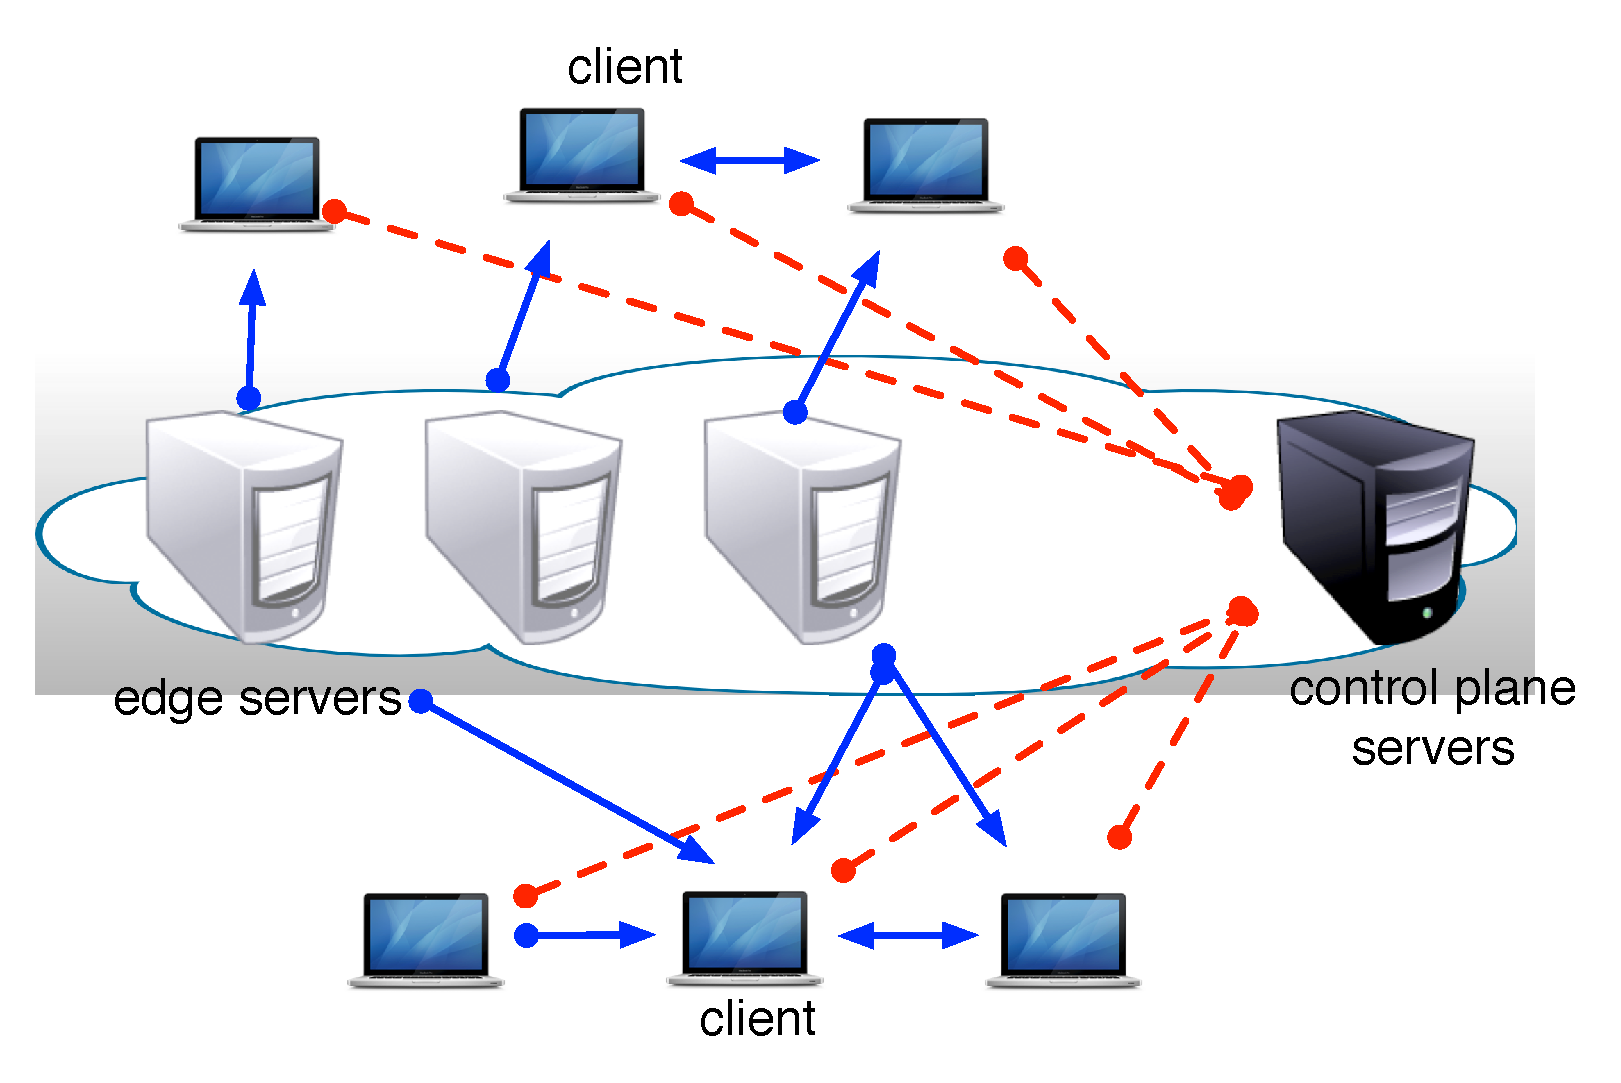
\includegraphics[scale=0.3]{graphs/netsession.eps}
\end{center}
\caption{Peer Assisted CDN Overview.}
\label{fig:p2pcdnoverview}
\end{figure} 




\section{Related Work}\label{relatedwork}
Content Distribution Networks with peer assist have been successfully deployed on the Internet, such as Akamai \cite{Zhao:2013:PCD:2504730.2504752}, \cite{Huang:2008:UHC:1496046.1496064} and LiveSky \cite{Yin:2010:LEC:1823746.1823750}.  
The authors of \cite{Zhao:2013:PCD:2504730.2504752} examine the risks and benefits of peer-assisted content distribution in Akamai and measure the effectiveness of its peer-assisted. 
The authors of \cite{Huang:2008:UHC:1496046.1496064} conclude from two real world traces that hybrid CDN-P2P can significantly reduce the cost of content distribution and can scale to cope with the exponential growth of Internet video content.  
Yin et al. \cite{Yin:2010:LEC:1823746.1823750} described commercial operation of a peer-assisted CDN in China.  
LiveSky solved several challenges in the system design, such as dynamic resource scaling of P2P, low startup latency, ease of P2P integration with the existing CDN infrastructure, and network friendliness and upload fairness in the P2P operation.  
Xu et al.\cite{DBLP:journals/corr/abs-1212-4915} using game theory, showed that the right cooperative profit distribution of P2P can help the ISP to maximize the utility.  
Their model can easily be implemented in the context of current Internet economic settlements.  
Misra et al.\cite{Misra:2010:IPS:1811099.1811064} also mentioned the importance of P2P architecture to support content delivery networks.
The authors use cooperative game theory to formulate simple compensation rules for users who run P2P to support content delivery networks.

The idea of telco- or ISP-managed CDN has been proposed in recent years.  
The complexity of the CDN business encourage telcos and ISPs to manage their own CDN, rather than allow others to run CDNs on their networks.  
It has been shown that it is cost effective \cite{federation}\cite{norton2011internet}. 
Kamiyama et al. \cite{NoriakiKAMIYAMA2013} proposed optimally ISP operated CDN.
Kamiyama et al. mentioned that, in order to deliver large and rich Internet content to users, ISPs need to put their CDNs in data centers.  
The locations are limited while the storage is large, making this solution effective, using optimum placement algorithm based on real ISP network topologies.  
The authors found that inserting a CDN into an ISP's ladder-type network is effective in reducing the hop count, thus reduce total link cost.  
Cisco has initiated an effort to connect telco- or ISP-managed CDNs to each other, to form a CDN federation \cite{federation} using open standards \cite{cdni}.  
They argue that the current CDN architecture is not close enough to the users and ISPs can fill this position.

The idea of utilizing the user's computation power to support ISP operation is not new.  
The Figaro project \cite{figaro} proposed residential gateway as an integrator of different networks and services, becoming an Internet-wide distributed content management for a proposed future Internet architecture \cite{figaro}.  
Cha et al.,\cite{Cha:2008:NTP:1855641.1855646} performed trace analysis and found that an IPTV architecture powered by P2P can handle a much larger number of channels, with limited demand for infrastructure compare to IP multicast.  
Jiang et al. \cite{Jiang:2012:OMD:2413176.2413193} proposed scalable and adaptive content replication and request routing for CDN servers located in users' home gateways.  
Maki et al.\cite{NaoyaMAKI2012} propose traffic engineering for peer-assisted CDN to control the behavior of clients, and present a solution for optimizing the selection of content files.
Mathieu et al., \cite{6249305} are using data gathered from France telecom network to calculate reduction of network load if customers are employed as peer-assisted content delivery.

Guo et al., \cite{1613869} is closest with our work because we use that work as comparison and we use author's utility function.
The author proposed local system (local counter) to calculate the segment popularity in peer-assisted proxy system. 
The author use popularity for proxy cache replacement strategy. 
In peer side, the author use utility function for cache replacement strategy.  
The utility function is also function from popularity.
While the authors successfully show that the results are very good, the peer-assisted system behavior over time is not explain because the author focus on local properties such as proxy cache size variations and peer cache size variations.
The explanation of the optimal number of replicas is not also clear because unavailable information when the snapshot is taken.  
In our work, we complement Guo et al., \cite{1613869} work with VoD viewing popularity evolution model and describe the behavior of the peer-assisted CDN over the time.


\section{Characterizing Internet VoD Popularity}\label{popularity}
Before analyzing the system description and video caching, we first examine the popularity characteristics of Internet VoD services.
We use YouTube as example of VoD service.
The studies of content popularity evolution are mostly considered in short time periods.
Borghol et al., \cite{Borghol:2011:CMP:2039452.2039717} measure the evolution of content popularity in long periods (36 weeks) in which view count statistics of Youtube. 
Complement with Borghol et al., \cite{Borghol:2011:CMP:2039452.2039717} work, we also did same measurement as Borghol et al., \cite{Borghol:2011:CMP:2039452.2039717} for eight weeks from October-November 2013.
We collected number of views, upload time YouTube videos on a weekly basis.
We use YouTube's API to sampling popular videos. 
The API provides a call that returns details on 20 popular videos.
Finally, we combine our datasets with Borghol et al.,\cite{Borghol:2011:CMP:2039452.2039717} datasets. 

In datasets, we have one-week spacing between consecutive snapshots.  
We can get how many times the video was view during the one-week period since last week or since snapshot $(i-1)$. 
As same Borghol et al., \cite{Borghol:2011:CMP:2039452.2039717} work, we define time-to-peak for a video as its age (time since upload) at which its weekly viewing rate is the highest during measurement (from the first week until end of measurement).
The time-to-peak distributions is shown in fig.\ref{fig:timetopeak}.
Figure \ref{fig:timetopeak} shows that around three-quarters of a large fraction videos peak within the first six weeks since their upload and beyond six weeks we have uniform distribution thus the time-to-peak is exponentially distributed mixture with uniform distribution. 
Our finding coherence with Borghol et al., \cite{Borghol:2011:CMP:2039452.2039717}.
To estimate the the rate parameter of exponential part of time-to-peak distribution, we use Maximum Likelihood Estimation (MLE) \cite{clauset2009power}.
Using MLE method, we can get exponential parameter $\lambda = 0.61$. 
For weekly views distribution, Borghol et al., \cite{Borghol:2011:CMP:2039452.2039717} found that beta distribution is a good model to explain video views evolution thus we follow Borghol et al., \cite{Borghol:2011:CMP:2039452.2039717} for  weekly views distribution model.

\begin{figure}[!t]
\begin{center}
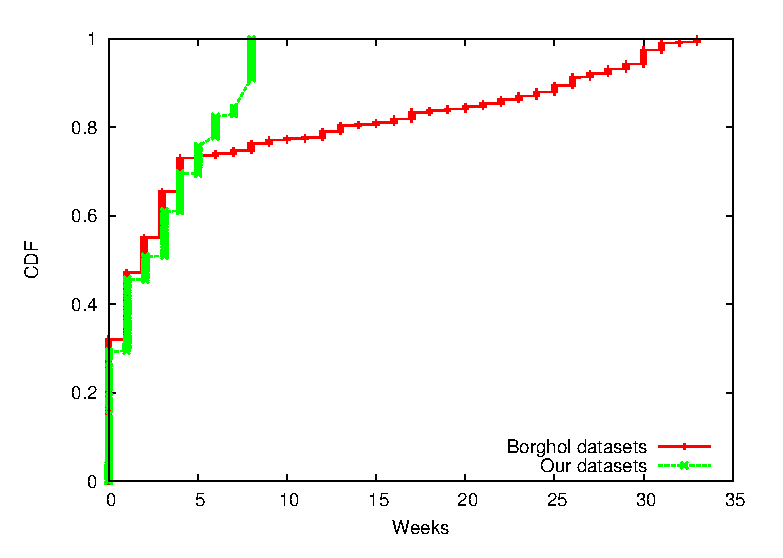
\includegraphics[scale=0.6]{graphs/timetopeak.eps}
\end{center}
\caption{Time to peak empirical distribution.}
\label{fig:timetopeak}
\end{figure} 



\section{System Description}\label{systemdescription}
In this paper, we consider a peer-assisted CDN system. 
There are two main components: (1) the CDN servers which at a minimum consist content delivery platform and control plane platform. 
(2) Clients which request and downloads the videos.
In addition, clients form a self-organized P2P overlay network.

The CDN servers are maintained by a CDN company or a content provider company (e.q Netflix) or an Internet service provider (ISP).
In peer-assisted CDN, a peer caches the videos that it has downloaded.
Peers independently manage their cache localy.
When a peer join the system video replica is cached.
When a peer leaves the system video replica is evicted. 
In both process, a peer always reports to CDN thus CDN knows the status of a peer.



\subsection{CDN caching strategy}\label{cdncachingstrategy}
As we mentioned in previous sect.\ref{systemdescription}, the CDN collects metadata.
The metadata will be used for assisting P2P clients for caching decision. 
The metadata that CDN collects are the following parameters:
\begin{itemize}
\item $n_j^r$: total number of the times video $j$ has been requested.  
\item $t_j^r$: the last time video $j$ was requested.
\item $n_j^s$: total number of the time that video $j$ is served by CDN.
\item $t_j^s$: the last time that video $j$ was served by CDN.
\item $a_j$: the time that video $j$ was added to video server's catalog.
\item $n_j^c$: total number of the times that video $j$ is served by CDN.
\item $t_j^p$: the time that video  is added into peer's cache.
\item $t$: the current time.
\end{itemize}

We use the method proposed in \cite{1613869} to estimate the popularity video as follows:

\begin{equation}
P_j = min\left\{\frac{n_j^r}{t_j^r - a_j}, \frac{1}{t - t_j^r}\right\}
\label{eq:videopopularityestimation}
\end{equation}

The expression of $\frac{n_j^r}{t_j^r - a_j}$ reflects the long-term request rate of the video or probability of future access rate and the expression of $\frac{1}{t - t_j^r}$ reflects the approximation of the video's recent request rate.
The video with the smallest popularity is chosen as the candidate to be replaced when the CDN cache is full. 
Since above eq.\ref{eq:videopopularityestimation} considering both recent access and pass access information, the CDN can cache the most requested video for clients.

\subsection{Peer caching strategy}\label{peercachingstrategy}
In a peer side, we follow Guo et al., \cite{1613869} for cache replacement strategy. 
We define the utility function for peer replacement as follows:

\begin{equation}
u = \frac{ (f(p)-f(p_{min})) \times  (f(p_{max})-f(p))}{r^{\alpha + \beta}}
\label{eq:utilityfunction}
\end{equation}

$p$ represents popularity of the video, $p_{min}$ represents estimation of minimum popularity in P2P system, $p_{max}$ represents estimation of maximum popularity in P2P system, $r$ represents the number of replicas of the video in the system, and $f(p)$ is monotonic non-decreasing function.
$\alpha$ and $\beta$ are the adjustment factor.

The CDN can calculate $p_{min}$ and $p_{max}$ then propagate to the P2P system.
We choose the video with the smallest $u$ value as the candidate to be replaced when a peer's cache capacity is full.
In the next section (sect.\ref{evaluation}), we will show how popularity evolution knowledge is used to simplified our calculation for utility function.

\subsection{Peer caching strategy}\label{peercachingstrategyproposal}
Equation \ref{eq:utilityfunction} express the utility function used by peer for cache replacement. 
Since we can estimate before-peak week, at-peak week, and after-peak week of video, we modified the utility function as follows: 
\begin{itemize}

\item In before-peak and after-peak phases, we assume that requests to video are low thus we only consider minimum popularity.
\begin{equation}
u = \frac{f(p)-f(p_{min})} {r^{\alpha+\beta}}.
\label{eq:utilityfunctionbeforeafter}
\end{equation}

\item In at-peak phase, we assume that request to video are high thus we only consider maximum popularity.  

\begin{equation}
u = \frac{f(p_{max})-f(p)}{r^{\alpha+\beta}}.
\label{eq:utilityfunctionat}
\end{equation}


\end{itemize}


\begin{figure}[!t]
\begin{center}
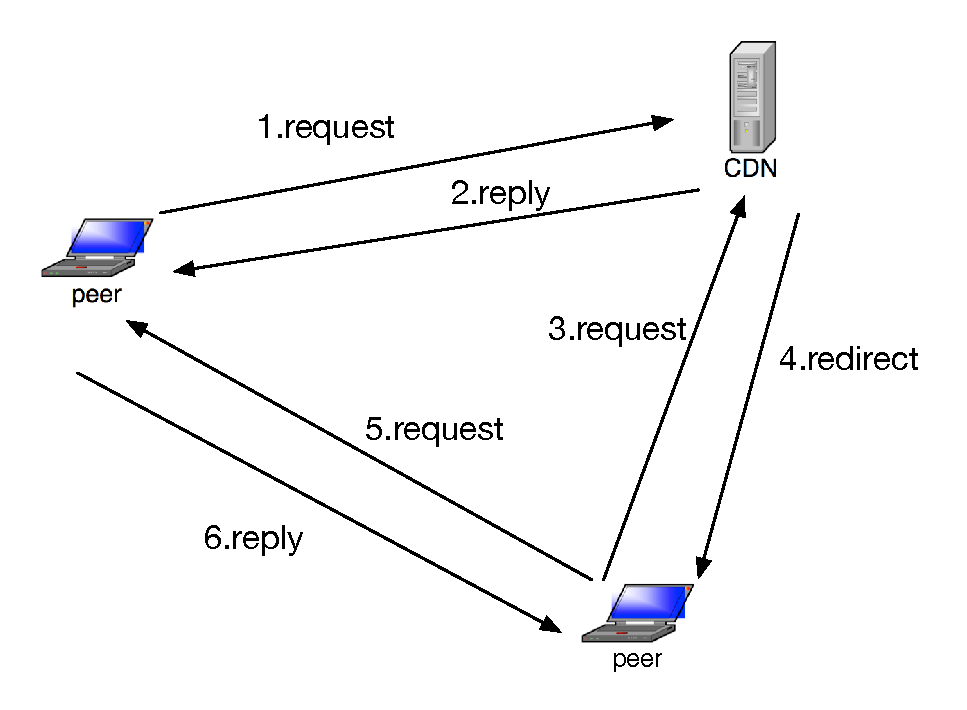
\includegraphics[scale=0.5]{graphs/p2p-system-description.eps}
\end{center}
\caption{Peer interaction in simulator.}
\label{fig:p2pcdninteractioninsimulator}
\end{figure} 


\section{Evaluation}\label{evaluation}
In order to evaluate the proposed cache strategy using before-peak, at-peak, and after-peak information from VoD model, we have to compare our model to PROP model \cite{1613869}.

\subsection{Simulation Design}\label{simulationdesign}
An event driven simulator is developed using Python for this purpose and we use Youtube VoD model as video catalog of the simulated Internet VoD system in our experiment.
In our simulator, time is divided into rounds. 
During a round, a peer request a video.



%%%contribution 500MB vs 1000MB CDN 10GB
\begin{figure*}[!t]
\centering
\subfloat[CDF percentage of contribution of peers where peer capacity 500MB and CDN capacity 10GB. $x$ and $y$ axis in logscale.\label{fig:peer500MBcontributionCDN10G}]{
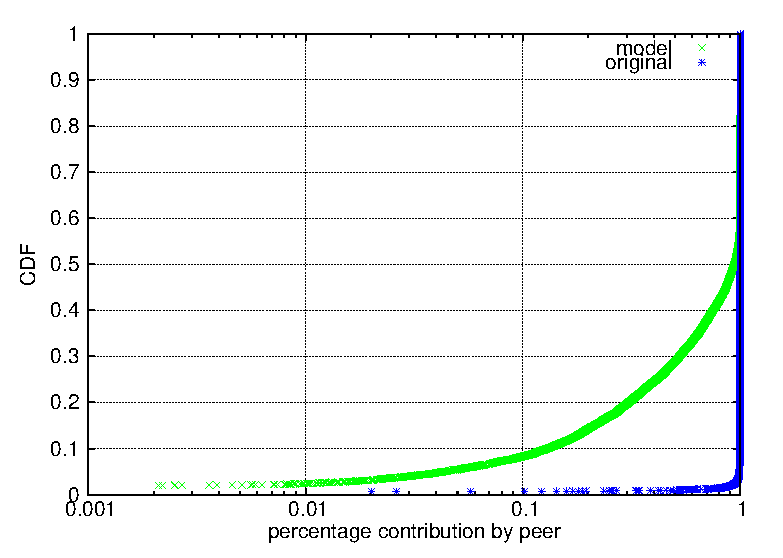
\includegraphics[width=5.7cm]{graphs/hit-model-original-1000MB-cdf-log.eps}
}
\hfill
\vspace{2mm}
\subfloat[CDF percentage of contribution of peers where peer capacity 1000MB and CDN capacity 10GB. $x$ and $y$ axis in logscale.\label{fig:peer1000MBcontributionCDN10G}]{
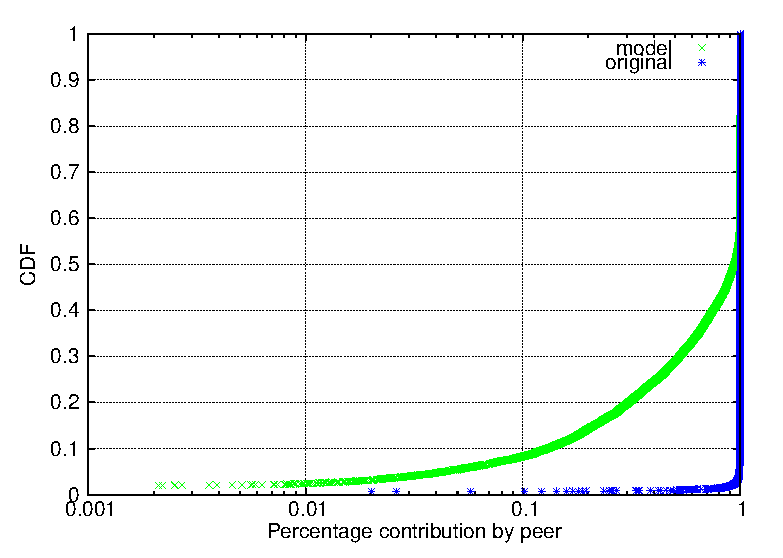
\includegraphics[width=5.7cm]{graphs/hit-model-original-500MB-cdf-log.eps}
}
\hfill
\subfloat[CDF peer contribution percentage between peer with 500MB capacity and 1000MB capacity and CDN capacity 10GB.\label{fig:peer500MB-vs-1000MBcontributionCDN10G}]{
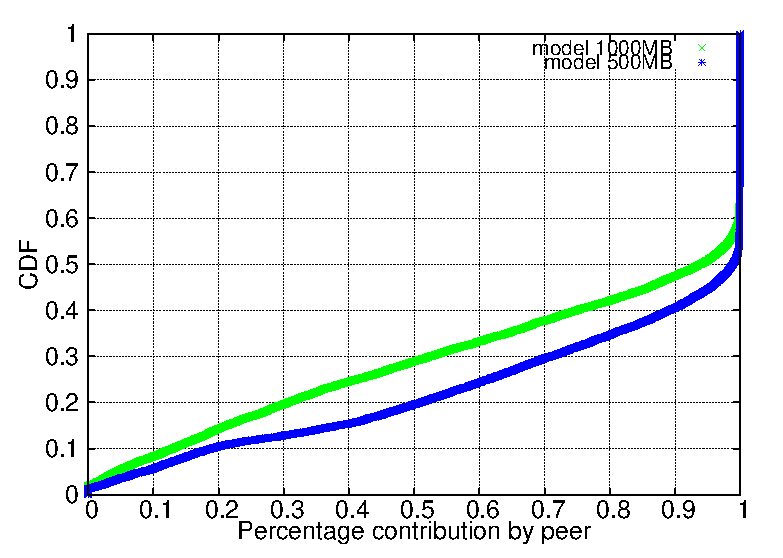
\includegraphics[width=5.7cm]{graphs/hit-model-500MBvs-1000MB-cdf.eps}
}
\vspace{2mm}
\caption{CDF peer contribution for peer capacity 500MB and 1000MB, CDN capacity 10000MB. Model refers to our work and original refer to PROP \cite{1613869}.}
\label{fig:peercontribution}
\end{figure*}


%%%contribution 500MB vs 1000MB CDN 20GB
\begin{figure*}[!t]
\centering
\subfloat[CDF percentage of contribution of peers where peer capacity 500MB and CDN capacity 20GB. $x$ and $y$ axis in logscale.\label{fig:peer500MBcontributionCDN20G}]{
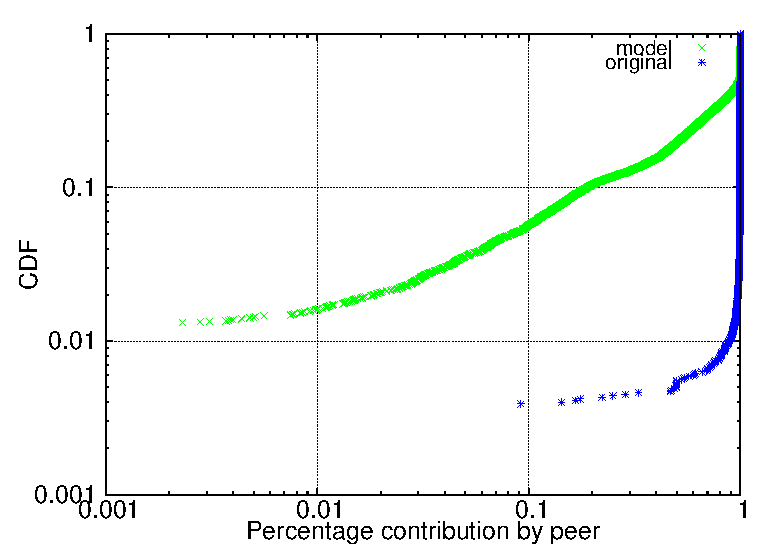
\includegraphics[width=5.7cm]{graphs/20G/hit-model-original-1000MB-20G-cdf-log.eps}
}
\hfill
\vspace{2mm}
\subfloat[CDF percentage of contribution of peers where peer capacity 1000MB and CDN capcity 20GB. $x$ and $y$ axis in logscale.\label{fig:peer1000MBcontributionCDN20G}]{
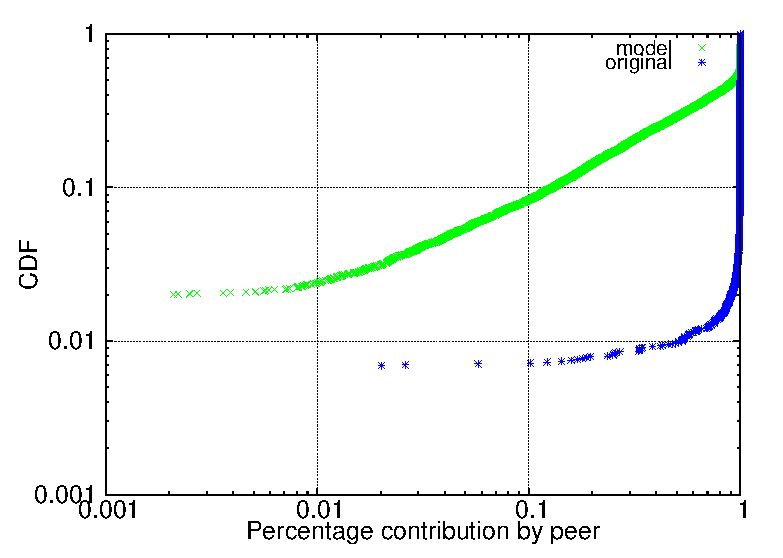
\includegraphics[width=5.7cm]{graphs/20G/hit-model-original-500MB-20G-cdf-log.eps}
}
\hfill
\subfloat[CDF peer contribution percentage between peer with 500MB capacity and 1000MB capacity and CDN capacity 20GB.\label{fig:peer500MB-vs-1000MBcontributionCDN20G}]{
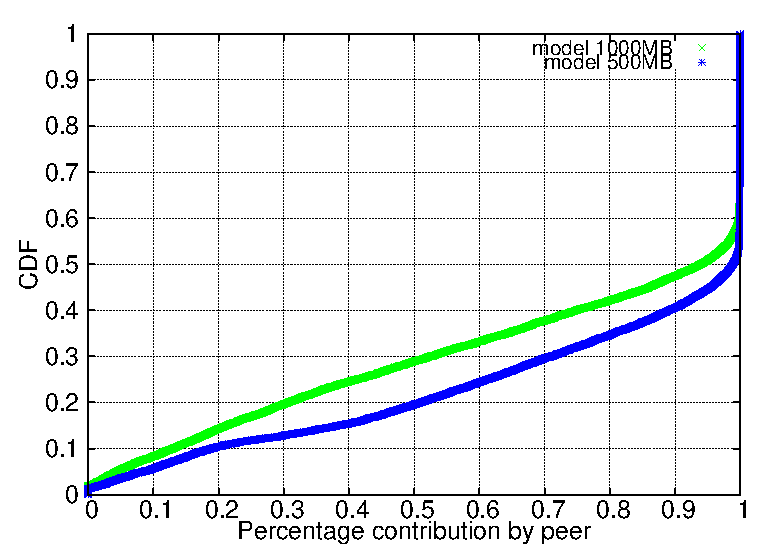
\includegraphics[width=5.7cm]{graphs/20G/hit-model-500MBvs-1000MB-20G-cdf.eps}
}
\caption{CDF peer contribution for peer capacity 500MB and 1000MB, CDN capacity 20000MB. Model refers to our work and original refer to PROP \cite{1613869}.}
\label{fig:peercontribution20G}
\end{figure*}

\begin{figure}[!t]
\begin{center}
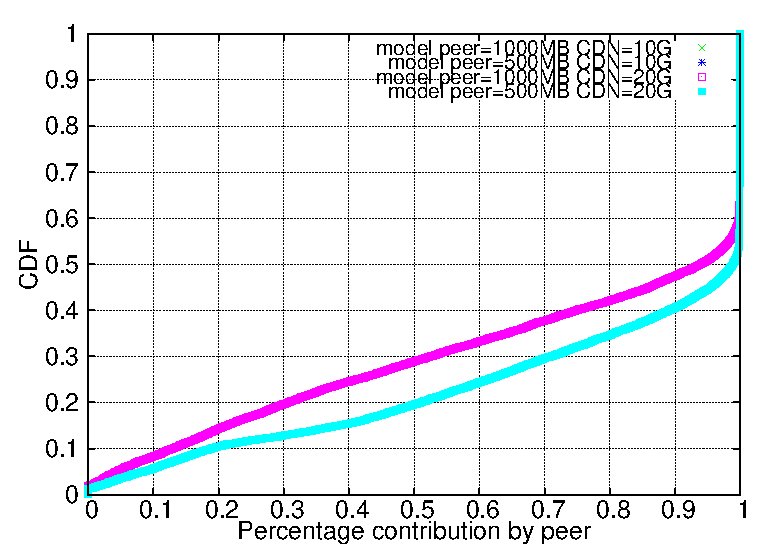
\includegraphics[scale=0.6]{graphs/hit-model-500MBvs-1000MB-10G-20G-cdf.eps}
\end{center}
\caption{Comparisan the model of CDN capacity 10GB vs. 20GB.}
\label{fig:10Gvs20G}
\end{figure} 



\begin{figure*}[!t]
\centering
\subfloat[Number of replicas by popularity at $t=10$day for peer capacity 500MB.\label{fig:peer500MBvs1000MBreplica10dayCDN10Gpopularity}]{
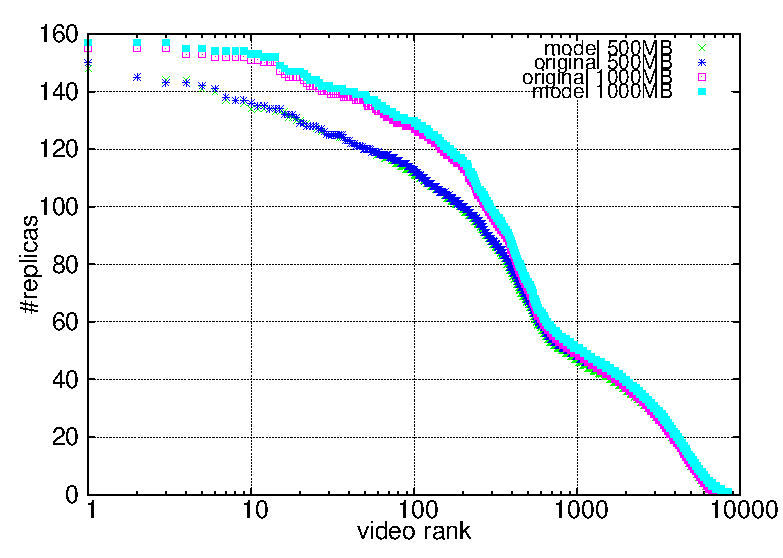
\includegraphics[width=5.7cm]{graphs/replica-10hari-500vs1000-log.eps}
}
\hfill
\subfloat[Number of replicas by popularity at $t=6$week for peer capacity 1000MB.\label{fig:peer500MBvs1000MBreplicaweek6CDN10Gpopularity}]{
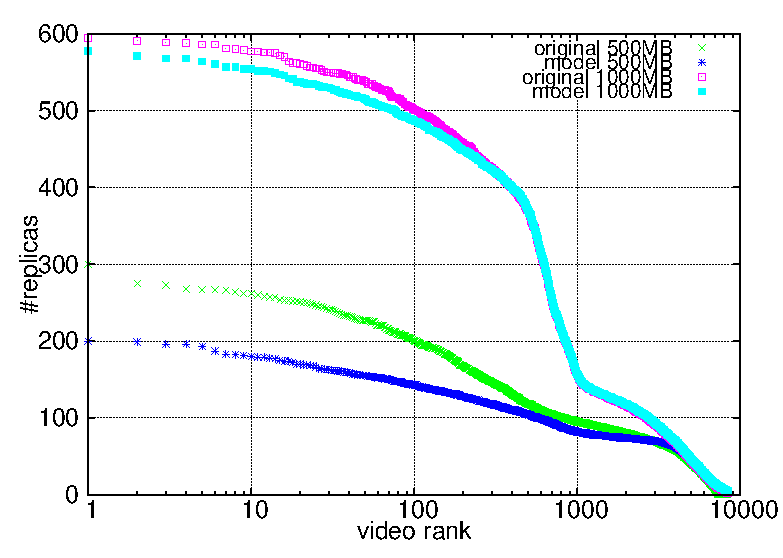
\includegraphics[width=5.7cm]{graphs/replica-minggu6-500vs1000-log.eps}
}
\subfloat[Number of replicas by popularity at $t=10$week for peer capacity 1000MB.\label{fig:peer500MBvs1000MBreplica10week10CDN10Gpopularity}]{
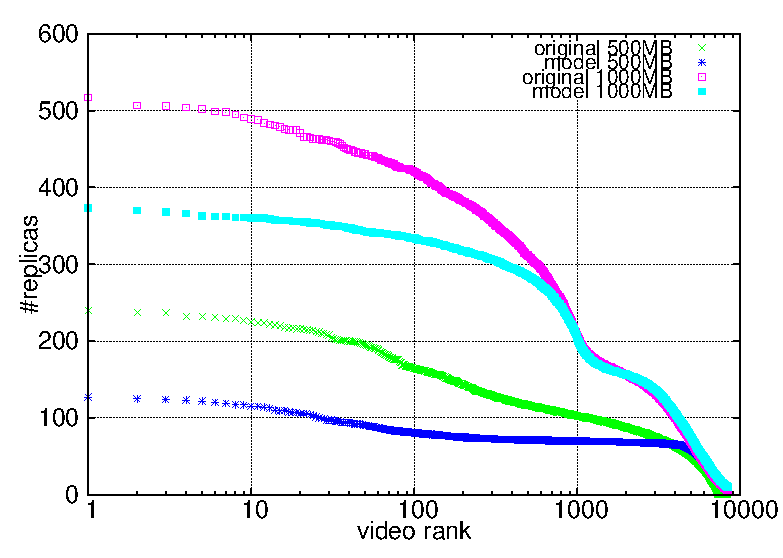
\includegraphics[width=5.7cm]{graphs/replica-minggu10-500vs1000-log.eps}
}
\caption{Distribution number of video replicas at snapshot $t=10$day, $t=6$week, and $t=10$week for peer capacity 500MB and 1000MB, CDN capacity 10GB.}
\label{fig:replicaatbypopularity}
\vspace{-2mm}
\end{figure*}

\begin{figure*}[!ht]
\centering
\subfloat[Number of replicas by popularity at $t=10$day for peer capacity 500MB and 1000MB, CDN capacity 20GB.\label{fig:peer500MBvs1000MBreplica10dayCDN20Gpopularity}]{
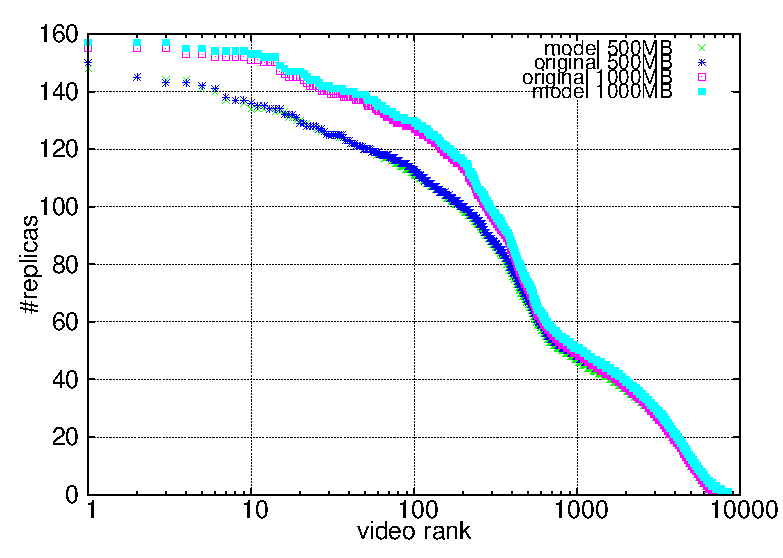
\includegraphics[width=5.7cm]{graphs/20G/replica-10hari-500vs1000-20G-log.eps}
}
\hfill
\subfloat[Number of replicas by popularity at $t=6$week for peer capacity 500MB and 1000MB, CDN capacity 20GB.\label{fig:peer500MBvs1000MBreplicaweek6CDN20Gpopularity}]{
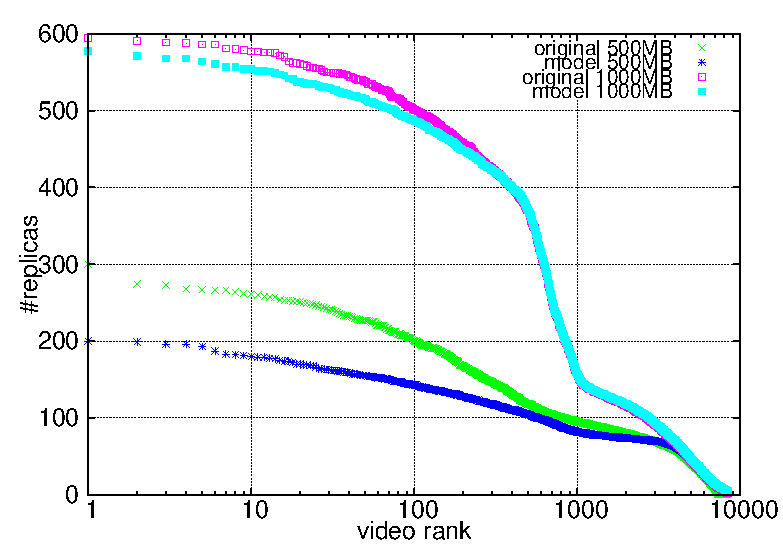
\includegraphics[width=5.7cm]{graphs/20G/replica-minggu6-500vs1000-20G-log.eps}
}
\subfloat[Number of replicas by popularity at $t=10$week for peer capacity 500MB and 1000MB., CDN capacity 20GB.\label{fig:peer500MBvs1000MBreplica10week10CDN20Gpopularity}]{
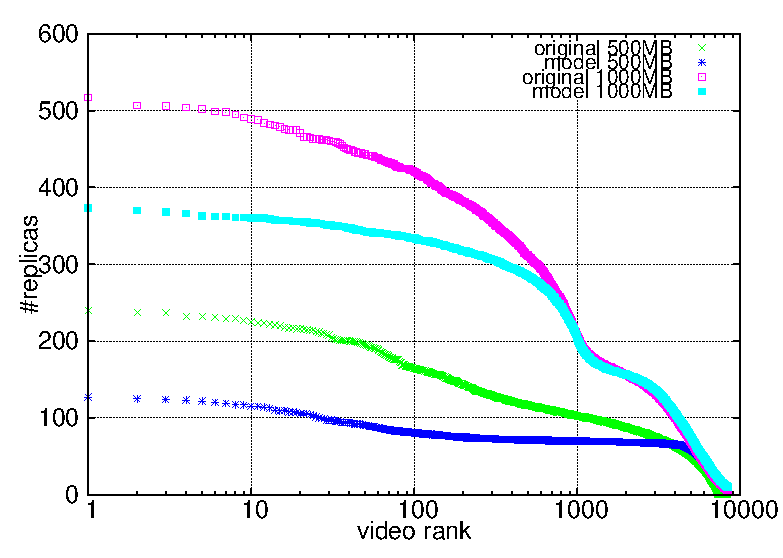
\includegraphics[width=5.7cm]{graphs/20G/replica-minggu10-500vs1000-20G-log.eps}
}
\caption{Distribution number of replicas at snapshot $t=10$day, $t=6$week, and $t=10$week for peer capacity 500MB and 1000MB, CDN capacity 20GB.}
\label{fig:replicaatbypopularity20G}
\vspace{-2mm}
\end{figure*}


\subsection{Peer and CDN server interaction}
In fig.\ref{fig:p2pcdnoverview}, we describe the process of a peer that requests a video in simulator.
peer and cdn are implemented in object oriented model. 
When a peer requests a video, it always goes to a CDN server (step 1). 
The CDN provides the videos to the peer (step 2). 
If there is another peer request same video, that request will go to CDN (step 3).  
CDN will check its record to see if there are some peers cache that requested video.  
If there are some peers cache that requested video, CDN will reply with redirect message that asking a peer to download requested video from other peer (step 4).
If there are no peers have requested video, CDN will serve the video.   
A peer then can request the video to other peer and get the video (step 5 and step 6).
From this description, we can see that deploying peer-assisted CDN can save some traffic since the clients which form P2P network can sharing the contents or videos.


\subsubsection{Catalog Generator}
In catalog generator, we assume peer request a video to CDN following poisson process with a mean rate $\lambda=1.1$ \cite{Zink:2009:CYN:1502814.1502987} and we made it 3600 videos per hour, finally we generate video request for 360 days of simulation thus we have 31104000 requests by peers. 
How a peer choice a video, we will explain in next paragraph.

First of all, we calculate the number of videos at-peak time as follows: sample $N$ value from the time-to-peak distribution and determine the number of videos $n_j^{at}$ that peak at week $j$. 
Total number of video $N = n_j^{before} + n_j^{at} + n_j^{after}$.\\
Next, we determine view count terminus which the number of final view count of video.
In view count terminus, we assume that a video will not get big additional view after at-peak phase.
We assign view count terminus randomly from datasets.
After determining view count terminus, we assign beta distribution parameter for every video. 

Since we can estimate the time of at-peak phase for each video, we know the mode of beta distribution value and we can calculate $\alpha$ and $\beta$ value using the mode of distribution formula: $m=\frac{\alpha-1}{\alpha + \beta - 2}$.  
We assign $\alpha$ value randomly between $1$ and $2$ thus we can calculate $\beta$ value.
With the knowledge of beta distribution of every video and its view count terminus, we can know the view count and view rate of every video as function from time.
The knowledge of view count and view rate, will be used top generate a video choice.  

For video choice, we estimate that a peer will choose video proportionally considering view count and view rate of the video.   
We can get view count and view rate from probability distribution function (PDF) and cumulative distribution function (CDF) of beta distribution above multiply by video's view count terminus.
In last step, we assign file size of video randomly between $1$MB and $200$MB.
Finally, we have a catalog that consists of: video to be chosen, time when uploaded, view count terminus, at-peak week, and video size.


\subsubsection{Simulation Parameters}
The simulation parameters are follows:
\begin{itemize}
\item Length: $360$ days.
\item Video size: random between $1$MB and $200$MB.
\item Peer capacity: [500MB,1000MB].
\item CDN capacity: $10000$MB and $20000$MB.
\item Number of peers: $100000$.
\item Number of videos: $10000$.
\end{itemize}
We compare our proposed improvement of PROP to original PROP \cite{1613869} implementation.



\subsection{Result and Discussion}\label{resultanddiscussion}

Figure~\ref{fig:peercontribution} shows CDF peer contribution for our model compare to PROP for peer capacity 500MB and 1000MB, with CDN capacity 20GB. 
One dot in a figure means how many percentage a video delivered by peers during simulation.z
Moreover fig.~\ref{fig:peer500MBcontributionCDN10G} shows the comparison of CDF of peer contributions between our model and PROP for peer capacity 500MB. 
Figure~\ref{fig:peer1000MBcontributionCDN10G} shows the comparison of CDF of peer contribution between our model and PROP for peer capacity 1000MB.
Figure~\ref{fig:peer500MB-vs-1000MBcontributionCDN10G} we compare our model between peer capacity 500MB and peer capacity 1000MB.
Peer capacity 1000MB gives higher peer contribution because additional space makes a peer can cache more videos.
From fig.~\ref{fig:peer1000MBcontributionCDN10G} and fig.~\ref{fig:peer500MB-vs-1000MBcontributionCDN10G}, We can see that our model can gain higher peer contributions than PROP.
We do significance statistical testing if our model has significantly different from PROP.
We use Kolmogorov-Smirnov (KS) test for this purpose.  
KS-test tries to determine if two datasets differ significantly.
It has the advantage of making no assumption about the distribution of data. 
KS-test reject the null hypothesis of no difference between datasets if $p$-value is small.
For peer capacity 500MB when we compare our model and PROP, we get $p$-value $0.5e-005$.
In peer capacity 1000MB case, we get $p$-value $0.46e-005$.
Because both $p$-values are below $1\%$, we can reject null hypothesis that both data are the same thus our results are significant.


Figure~\ref{fig:peercontribution20G} shows CDF peer contribution for our model compare to PROP for peer capacity 500MB and 1000MB, with CDN capacity 20GB.
Figure~\ref{fig:peer500MBcontributionCDN20G} shows the comparison of CDF of peer contributions between our model and PROP for peer capacity 500MB.
Figure~\ref{fig:peer1000MBcontributionCDN20G} shows the comparison of CDF of peer contributions between our model and PROP for peer capacity 1000MB.
From fig.~\ref{fig:peercontribution20G} and fig.~\ref{fig:peer500MBcontributionCDN20G} show that our model can gain higher peer contributions than PROP.
We also do significance statistical testing for both cases.  
We get $p$-value $0.5e-005$ for peer capacity 500MB case and $p$-value $0.47e-005$ for peer capacity 1000MB case.
Because the $p$-values less than $1\%$, therefore the results are signifincant.
Finally, fig.~\ref{fig:peer500MB-vs-1000MBcontributionCDN20G} shows the comparison between peer capacity 500MB and peer capacity 1000MB in our model. 
This figure shows that peer capacity 1000MB gives more contributions than peer capacity 500MB because additional space in peer makes a peer can cache more videos.  
Lastly, we compare our model peer capacity 500MB and 1000MB with CDN capacity 10GB and 20GB in fig.~\ref{fig:10Gvs20G}.
We found that there are no many different thus CDN capacity does not affect peer contributions. 


Figure~\ref{fig:replicaatbypopularity} shows distribution of the number of replicas at snapshot $t=10$day, $t=6$week, and $t=10$week ranked by video popularity for peer capacity 500MB and 1000MB, CDN capacity 10GB between our model and PROP.
Figure~\ref{fig:peer500MBvs1000MBreplica10dayCDN10Gpopularity} shows distribution of the number of replicas comparison for peer capacity 500MB and 1000MB and CDN capacity 10GB sorted by popularity rank at snapshot $t=10$day.
This figure shows that on snapshot $t=10$day there are no many different for peer capacity 500MB between our model and PROP except for peer capacity 1000MB PROP has lower number of replicas than our model for popular video rank between $1$ until $1000$ beyond that the number of replicas is same.
Figure~\ref{fig:peer500MBvs1000MBreplicaweek6CDN10Gpopularity} shows distribution of the number of replicas comparison for peer capacity 500MB and 1000MB and CDN capacity sorted by popularity rank at snapshot $t=6$week.
Both peer capacity 500MB and 1000MB show that our model has lower number of replicas compare to PROP for popular video rank between $1$ and $1000$ for peer capacity 500MB while for peer capacity 1000MB our model gives lower replicas for popular video rank between $1$ and $400$.  
Peer capacity 1000MB gives higher replicas than 500MB because additional capacity make more room for peer to cache videos.
Figure~\ref{fig:peer500MBvs1000MBreplica10week10CDN10Gpopularity} shows distribution of the number of replicas comparison for peer capacity 500MB and 1000MB and CDN capacity 10GB sorted by popularity rank at snapshot $t=10$week.
Again, our model gives lower number of replicas compare to PROP. 
Snapshot $t=10$ weeks gives lower number of replicas than snapshot at $t=6$week because in our model the utility function knows that $t=10$week is at after-peak phase thus the model only considering minimum popularity for all videos. 





\section{Conclusion and Future Work}\label{conclusion}
This paper presents a scheme for a ISP managed peer-assisted CDN model that 
Some areas of improvement that we have identified for future are:
We are also very interested to include energy trade off this peer-assisted CDN architecture in order to know how much energy saving by ISP and how much increase of energy at users home gateway side in this architecture.


% use section* for acknowledgement
\section*{Acknowledgment}
The authors would like to thank Internet research laboratory member at Keio University and anonymous reviewer.





% trigger a \newpage just before the given reference
% number - used to balance the columns on the last page
% adjust value as needed - may need to be readjusted if
% the document is modified later
%\IEEEtriggeratref{8}
% The "triggered" command can be changed if desired:
%\IEEEtriggercmd{\enlargethispage{-5in}}

% references section

% can use a bibliography generated by BibTeX as a .bbl file
% BibTeX documentation can be easily obtained at:
% http://www.ctan.org/tex-archive/biblio/bibtex/contrib/doc/
% The IEEEtran BibTeX style support page is at:
% http://www.michaelshell.org/tex/ieeetran/bibtex/
%\bibliographystyle{IEEEtran}
% argument is your BibTeX string definitions and bibliography database(s)
%\bibliography{IEEEabrv,../bib/paper}
%
% <OR> manually copy in the resultant .bbl file
% set second argument of \begin to the number of references
% (used to reserve space for the reference number labels box)
\bibliographystyle{IEEEtran}
\bibliography{manu}

% that's all folks
\end{document}


